\documentclass[11pt]{article}
\usepackage{pgf}
\usepackage{todonotes}
\usepackage{float}
\usepackage[american]{babel}
\usepackage{csquotes}
\usepackage[hypcap=true]{caption}
\usepackage{subcaption}
\usepackage[backend=biber,style=apa,url=false]{biblatex}
\DeclareLanguageMapping{american}{american-apa}
\bibliography{bibevol4.bib}
\usepackage{sgame}
\usepackage{tikz}
\usepackage{pgfplots}
 % Useful for Physics related math
\usepackage{physics}
\usepackage{amsmath}
\usepackage{amssymb} 
\usepackage{amsthm}
        % packages that allow mathematical formatting
\usepackage{setspace}
\setlength\parindent{0pt}
        % set space and indent and indent
\usepackage{hyperref}
\hypersetup{
            colorlinks,
                linkcolor={red!50!black},
                    citecolor={blue!50!black},
                        urlcolor={blue!80!black}
                }
\usepackage[a4paper,width=150mm,top=25mm,bottom=25mm]{geometry}

% New commands
\let\conju\overline
\newcommand\numberthis{\addtocounter{equation}{1}\tag{\theequation}}
\newcount\colveccount
\newcommand*\colvec[1]{
        \global\colveccount#1
        \begin{pmatrix}
                \colvecnext
        }
        \def\colvecnext#1{
                #1
                \global\advance\colveccount-1
                \ifnum\colveccount>0
                \\
                \expandafter\colvecnext
                \else
        \end{pmatrix}
        \fi
}
        % Columnvectors
\newtheorem{mydef}{Definition}

\pgfplotsset{compat=1.11}
\linespread{1.5}
\newcommand{\natnumb}{\mathbb{N}}
\newcommand{\realnumb}{\mathbb{R}}
\presetkeys{todonotes}{color=yellow,size=\scriptsize}{}
\def\stackedpayoffs#1#2{%
\begin{array}{rl}#1&\\[1.6mm]&#2\end{array}
}
\renewcommand\vec{\mathbf}
\usepackage[toc,page]{appendix}
\usepackage[utf8]{inputenc}
\usepackage{hyphenat}
%%%%%%%%%%%%%%%%%%%
%
% Make math nomenclatur  
\usepackage{nomencl}
\makenomenclature
\begin{document}
\nomenclature{$I$}{Set of players}%
\nomenclature{$\mathbb{S}$}{Set of pure strategies}%
\nomenclature{$S_i$}{Individual set of pure strategies for player $i$}%
\nomenclature[F]{$F$}{Pure strategy payoff function of the game}%
\nomenclature[F]{$F_i(\cdot)$}{Pure payoff function for player $i$}%
\nomenclature{$\Gamma(\cdot,\cdot,\cdot)$}{A game in normal form}
\nomenclature{A,B}{Payoff matrices of the row and the column player,% 
respectively}%
\nomenclature{$\Delta_i$}{Mixed strategy space of player $i$}%
\nomenclature[F]{$\hat{F}(\cdot,\cdot)$}{Mixed strategy payoff function}%
\nomenclature[b]{$\beta_i(y)$}{Best-reply for player $i$ against strategy $y$}%
\nomenclature[x]{$\vec{x}(t)$}{Population state vector at time $t$}%
\nomenclature{$x_i(t)$}{Share of population choosing strategy $i$ at time $t$}
\nomenclature[F]{$\hat{F}^i$}{Expected payoff of an individual with strategy $i$
against the population state $\vec{x}(t)$ at time $t$}
\nomenclature{$\rho_{ij}$}{Conditional switch rate for switching from 
strategy $i$ to strategy $j$}
\nomenclature[x]{$\varphi(x)$}{The polynominal of the replicator dynamic}
\nomenclature[e]{$\bar{\epsilon}$}{Invasion barrier}
\nomenclature[x]{$x_0$}{Initial condition for a dynamical system}
\nomenclature[F]{$\bar{F}(\vec{x}(t))$}{Average payoff across at the 
population state at time $t$}
\nomenclature[R]{$\realnumb$}{Real numbers}
        

%%%%%%%%%%%%%%%%%%%%%%
%
% Title page
\vskip 2cm
\thispagestyle{empty}
\vspace*{15mm}
\begin{center}
	\textbf{\Huge An evolutionary analysis of the stag hunt game}\\
    \vspace{5mm}
    \textbf{\large Eine evolutionäre Analyse des Hirschjagdspiels}\\
    \end{center}
\begin{center}
\vskip 0.5cm
	\large Bachelor Thesis \\	
\vskip 1.5cm	
	submitted to:
\vskip 1cm
Professor Dr. Matthias Blonski\\
Chair of Microeconomics\\
Faculty of Economics and Business Adminstration\\
Goethe University Frankfurt\\
Frankfurt am Main
\vskip 1cm
by:  \\
\vskip 0.5cm
Daniel Mairhofer\\
Trommstraße 25\\
68163 Mannheim\\
Tel.:\ +49 176 28567855 \\
Email: dmairhofer94@gmail.com\\
Student ID number: 5600126\\
Bachelor in Economics and Business Administration 
\end{center}
\vskip 1.5cm
\begin{center}
\large{06.06.2017} \\
\large{Frankfurt am Main}
\end{center}




\newpage
%
%%%%%%%%%%%%%%%%%%%%%%
%
% Table of figures
%
\pagenumbering{roman}
\tableofcontents
\newpage
\listoffigures
\newpage
%%%%%%
% Math abbreviation glossary
\renewcommand{\nomname}{Notation Index}
\printnomenclature[5em]
%%%%%%%%%%%%%%%%%%%%%%
\newpage
\pagenumbering{arabic}

%%%%%%%%%%%%%%%%%%%%%%
%
% Introduction
%
\section{Introduction}
%%%%%%%%%%%%%
%
%
% Introduction
%
%
%%%%%%%%%%%%%
The beginning of game theory dates back to Johann von Neumann in 1928,
who developed a mathematical framework
for modelling situations with strategic interactions of rational agents 
\parencite{v._neumann_zur_1928}.
In a situation of strategic interaction, the outcome for an agent does not
only depend on his choice, but also on the choice of the other agents.
In economics, such situations often present themselves as a social dilemma,
a situation where a group of agents is prevented to achieve the best
outcome for the group, because of strategic considerations of the individual
agent.

Asking a social scientist about \textit{the} example of a social dilemma, 
one usually gets to hear the story about two prisoners, arrested and 
seperately interrogated by an authority. Lacking the amount of evidence to sue 
the criminals for serious crimes, the authority offers them a deal 
simultaneously.
A confession would grant a prisoner amnesty and hence, he could escape the 
punishment for the serious crimes. However, if both chose to confess, 
they receive the
full sharpness of the law. Not admitting the crimes would leave the authority
with too little evidence, resulting only in a sentence for minor crimes.
This story, developed by Albert Tucker in 1950 and suitably named Prisoner's
Dilemma (PD) is usually represented in a table, as shown in figure \ref{fig:pd}, with
the options for each prisoners denoted by C, remaining silent, and D, admitting
their crimes. 
\begin{figure}[h]
        \centering
        \def\gamestretch{2.1}
        \begin{game}{2}{2}[Player 1][Player 2] & $C$ & $D$
                \\ $C$ &$\stackedpayoffs{-1}{-1}$ &$\stackedpayoffs{-4}{\phantom{-}0}$
        \\ $D$ &$\stackedpayoffs{\phantom{-}0}{-4}$ &$\stackedpayoffs{-3}{-3}$ \end{game}
\caption[Prisoner's Dilemma]{A parametrized representation of the prisoners dilemma}
\label{fig:pd}
\end{figure}
The total amount of years for the group is lowest if both do not confess, 
but each individual prisoner has the 
incentive to take the deal of the authority as this leaves him, independently
of what his fellow prisoner does, with a shorter time in prison. The dilemma 
clearly consists of the conflict between individual interest and 
the benefit of the group \parencite{skyrms_stag_2004}. 

Skyrms argues that there is ``another story that became a game'' 
which describes a different but underrepresented social dilemma
\parencite[1]{skyrms_stag_2004}. 
In \textit{A Discourse on Inequality}, 
Rousseau outlines the situation of hunters, heading out to hunt 
stag. However, if a hare runs past a hunter, he might consider to
shoot the hare, scaring of all stags in the forest. The total reward for
the group is surely lower, but it is rationale for the single hunter if he
expects the others to act the same, given the opportunity. In contrast
to PD, it is not the hunters individual interest that is competing with the
benefit of the group, but the uncertainty about what the other hunters choose
to do. In fact, none of the hunters would mind his choice
not to shoot a hare when returning with a stag, as his personal benefit is 
greater with a stag as bounty. 
\begin{figure}[h]
\begin{subfigure}{0.5\textwidth}
\begin{center}
        \def\gamestretch{2.1}
        \begin{game}{2}{2}[Player 1][Player 2] & $S$ & $H$
                \\ $S$ &$\stackedpayoffs{5}{5}$ &$\stackedpayoffs{0}{4}$
        \\ $H$ &$\stackedpayoffs{4}{0}$ &$\stackedpayoffs{3}{3}$ \end{game}
\end{center}
\caption{Numerical example}
\label{fig:numericalsh}
\end{subfigure}
\begin{subfigure}{0.5\textwidth}
\begin{center}
        \def\gamestretch{2.1}
        \begin{game}{2}{2}[Player 1][Player 2] & $S$ & $H$
                \\ $S$ &$\stackedpayoffs{a}{a}$ &$\stackedpayoffs{b}{c}$
        \\ $H$ &$\stackedpayoffs{c}{b}$ &$\stackedpayoffs{d}{d}$ \end{game}
\end{center}
\caption{Parametrized: $a > c \geq d > b$}
\label{fig:parash}
\end{subfigure}
\caption[Stag hunt game]{The stag hunt game: Numerical 
example and parametrized}
\label{fig:sh}
\end{figure}
Figure \ref{fig:sh} represents this dilemma 
for two hunters with a numerical example and parametrized. 
When both coordinate on stag hunting, denoted by S, they receive 
$5$. If one of them decides to shoot the hare, he gets $4$, whereas
the other hunter is left with nothing. Coordination on hare
hunting yields both with $3$. Clearly, hunting hare is safer as it yields 
a hunter at least with $3$, whereas stag hunting may leave a hunter with 
nothing. In the representation with parameters in figure
\ref{fig:parash}, these 
are usually assumed to satisfy the condition $a > c \geq d >b$. The 
relevance of this restriction will be discussed throughout the text.
Game theory calls this kind of game a coordination game.

In both outcomes, collective stag hunting and collective hare hunting,
each individual hunter has no incentive to change his action.
Hence, both outcomes are what game theory calls a Nash-equilibrium, originally
formulated by John Nash in 1950 \parencite{nash_equilibrium_1950}. In a 
Nash equilibrium all players of a game choose a best reply against
the strategies of the other players, so that none of them has an incentive
to deviate unilateral from his decision. Although this is the mainly used
solution concept, it does not give a definite answer in the stag hunt game.
One might argue that both hunters can speak to each other beforehand and
assure each other that hare hunting is more attractive to both them. 
However, \textcite{camerer_behavioral_2003}
argues that empirical observation and theory suggest that the problem is 
not solved that easily .
Furthermore, in a wide range of economic applications interaction of agents
happen repeatedly. Analyzing repeated prisoner dilemmas, it turns 
out that the resulting game can actually be interpreted as a stag-hunt game with
two Nash equilibria \parencite{skyrms_stag_2004}.

The connection between these two social dilemmas advocates that
the selection of equilibria should be investigated more deeply. 
An interesting approach to the equilibrium selection problem comes from
biology. Evolutionary game theory was pioneered by Maynard J. Smith and George
R. Price with their work on the conflict of animals in populations 
\parencite{smith_lhe_1973}. Started as a refinement of the Nash equilibrium,
the concept of an evolutionary stable strategy, various other authors, for 
example \textcite{taylor_evolutionary_1978}, \textcite{hofbauer_note_1979} and
\textcite{zeeman_dynamics_1981}, developed a `time dependent dynamical
extension of game theory'' \parencite[55]{hanauske_evolutionare_2011}.
In contrast to traditional game theory, the evolutionary approach  models
agents in a large population, interacting repeatedly in a strategic environment. 
Furthermore, the agents are not assumed to be rational, but follow a specific 
rule, updating their strategy. 
As outlined in the rest of this thesis, the
evolutionary approach offers a possible answer to the coordination
problem in the stag hunt game.

The thesis is organized as follows. Section 2 introduces the 
framework of traditional game theory for the stag hunt game and discusses
the traditional approach to the equilibrium selection problem. Section 3
introduces evolutionary game theory and presents the replicator dynamic. 
Later on, it will be discussed how the evolutionary approach selects
between multiple equilibria. Section 4 demonstrates the effect of a
network externality in the underlying framework. Looking for evidence on
how real people play the stag hunt game, section 5 considers experimental
literature on the topic. Section 6 concludes and shows the application of
evolutionary game theory and the stag hunt game in economics.


%
%%%%%%%%%%%%%%%%%%%%%%
%
% The traditional stag hunt game
%
\section{The Stag Hunt Game}
\label{sec:traditional}
As already explained, the stag hunt game is played by 
two players who choose their
strategies simultaneously.
Both have information about the strategies of the
other player and the payoffs they and their opponents receive. In game theory
such a game is called a \textit{normal form} game with complete information. 
Typically, such a game is formalized as a Triplet $\Gamma = (I,\mathbb{S},F)$, 
with the set of players $I=\{1,2,...,n\}$, where $n \in \mathbb{N}$ is the 
total number of players. 
Expressing all possible states of the game, the pure
strategy space of the game $\mathbb{S}$ is defined as the cartesian
product of the individual pure strategy spaces $S_i$ for a player $i \in I$,
$\mathbb{S}=\times_i S_i$. The individual pure strategy space is defined as
$S_i = \{1,2,...,m_i\}$, where $m_i \in \mathbb{N}$ denotes the total 
number of strategies available to player $i$. 
The payoff 
function of the game is denoted by $F: S \rightarrow \realnumb^n$.
As this text focuses upon the stag hunt game, these definitions reduce to the 
following.
By setting $n=2$, we define the set of two hunters playing SH as $I=\{1,2\}$. 
In the SH game, each hunter can choose one out of two pure strategies, namely, 
hunting stag (strategy 1 or S) or hunting hare (strategy 2 or H).
Therefore, the pure strategy space is defined by $S_i = \{1,2\}$, which results
by setting $m_i=2$. 
The strategies are called pure to distinguish
them from the later introduced mixed strategies. 
In the SH game both players choose from
the same set of strategies such that $S_1 =S_2=S$. Combining the strategy spaces
of the two players with the cartesian product
yields the definition of the pure strategy space of the game
$\mathbb{S}= S \times S = S^2$. Games played by two players with two strategies
each, are often said to be 2x2 games.    

Considering the story Rousseau told, the hunters do not just hunt
for their pleasure, but to sell their loot for a reward or to feed their 
families. 
This is captured by the definition of an individual payoff function for player
i, $F_i:S \rightarrow \realnumb$, which maps a payoff $F_i(s) \in \realnumb$ 
to every state of the game $s=(s_1,s_2) \in S^2$, where $s_i$ is a pure
strategy of player $i$. A state of the game $s$ is sometimes simply called 
strategy profile.
The payoffs are usually interpreted as \textit{von-Neumann} utility when 
played by individuals or households and may be interpreted as earnings 
regarding firms \parencite{fudenberg_theory_1998}. 

In the special case of two players, one can define a payoff matrix for
player 1, $A \in \realnumb^{2 \times2}$ and for player 2,
$B \in \realnumb^{2 \times2}$. The elements of the matrices $A_{kl}$ and
$B_{kl}$ state the payoffs to the players for a given strategy profile. 
Hence, the elements are defined as $A_{kl}= F_1(k,l)$ and 
$B_{kl} =F_2(k,l)$ with the pure strategies $k,l \in S$.
Using the 
representation in figure \ref{fig:parash}, one can identify the 
payoff matrices for the players as
\begin{align}
     A = \mqty(a && b \\ c && d), \quad B = \mqty(a && c \\ b && d).
        \label{eq:matrix}
\end{align}
For the SH game studied in this thesis, the following definition is important: 
\begin{mydef}
        A two player game $\Gamma=(I,S_1 \times S_2, A,B)$ is called symmetric
        if the players of the game have the same strategy space $S_1=S_2=S$ and
        for the payoff matrices the condition $B=A^T$ holds. Therefore, the
        game is well-defined as $\Gamma=(I,S^2,A)$.
        \label{symmetry}
\end{mydef}
Clearly, the SH game satisfies this condition. Both hunters have the same 
strategies available and the payoff matrices defined in equation
\eqref{eq:matrix} are the transpose of the other.
Hence, it is irrelevant which player is labeled as player 1 or 2, because 
they are identical with respect to their strategies and payoffs.

Usually a game is extended by the possibility of the players to play
\textit{mixed strategies}. 
Intuitively, the hunters in the SH game could  
choose whether to shoot the stag or the hare by using a randomization
tool such as flipping a coin. However, randomization is not really
satisfying in most applications \parencite{radner_private_1982}. An
alternative interpretation, outlined by Rubinstein, is that mixed 
strategies are actually deterministic, but seem to be random because they 
depend on not modelled private information of the individuals 
\parencite[914]{rubinstein_comments_1991}. In the evolutionary context,
discussed in section \ref{sec:evolutionarystaghunt}, mixed strategies have
a different, unproblematic interpretation. Apart from the interpretation 
problem, mixed strategies are appealing because they ensure the existence
of a Nash equilibrium, which is defined later in section 
\ref{sec:traditionalconcepts}.
Formally, every player of the game assigns a probability distribution over
his pure strategies space. A strategy $x_i \in \Delta_i$ of 
player $i \in I$ is called a \textit{mixed strategy}, where $\Delta_i$ is 
the mixed strategy space 
\begin{align*}
        \Delta_i = \{ x_i = (x_{i1}, x_{i2})^T \in \realnumb^2 : 
                \sum_{k=1}^2 x_{ik} = 1, x_{ik} \geq 0 \quad
\forall k \in S\}.
\end{align*}
In a symmetric game, the mixed strategy spaces of the players are
equal, as both players are not restricted in assigning probabilities to their
pure strategies. For the SH game this means $\Delta_1 = \Delta_2 = \Delta$.
With this notation, a pure strategy can be interpreted as a mixed strategy,
that assigns probability one to the pure strategy chosen and zero to all
other strategies. This is represented by the unit vectors 
$e_k \in \Delta$, where $k \in \{1,2\}$. 
Hence, $e_1 = (1,0)^T$ is the pure strategy hunting stag 
and $e_2 =(0,1)^T$ denotes the pure strategy hunting hare.
The combined mixed strategy space of the game is $\Delta^2 = \Delta \times
\Delta$.
From now on, except otherwise indicated, $x \in \Delta$ 
denotes a (mixed) strategy
chosen by player 1 and $y \in \Delta$ a (mixed) strategy of player 2.
Again, similar to the pure strategy case, the mixed strategy payoff 
$\hat{F}_i:\Delta^2 \rightarrow \realnumb$ maps 
any state in the mixed strategy
space  $(x,y) \in \Delta^2$ to an expected payoff 
$\hat{F}_i(x,y) \in \realnumb$.
With the matrix notation this is defined as: 
\begin{alignat*}{2}
        \hat{F}_1(x,y) &= x^T A y \\
        \hat{F}_2(x,y) &= x^T A^T y 
\end{alignat*}
Summarizing the notation, the SH game can be defined as a symmetric two-player
normal form game $\Gamma = (I=\{1,2\}, \Delta^2, \hat{F})$.

\subsection{Solution Concepts}
\label{sec:traditionalconcepts}
In describing the behavior of agents, game theory developed a wide range of 
tools to solve these strategic interactions. First of all, for each individual
a best-reply is defined by simply describing the strategies available to the
agent which yield the highest expected payoff against a given 
strategy of the other player.
Formally, the \textit{best-reply} $\beta_i(y)$ for player $i \in I$ to a 
strategy $y \in \Delta$ played by $j \neq i$ is defined as:
\begin{align}
        \label{eq:bestreply}
        \beta_i(y) = \{x \in \Delta: \hat{F}(x,y) \geq \hat{F}(x',y), 
        \quad \forall x' \in \Delta\}
\end{align}
Based on agents choosing a best-reply, the most frequently 
used solution concept of
a normal form game is the \textit{Nash equilibrium}.
The Nash equilibrium was named by its proposer John Nash in 1950 
and due to its prominence it is sometimes simply referred to as equilibrium 
or NE.
In the following, the definition of a Nash equilibrium in a two
player normal form game is stated. 
\begin{mydef}
        \label{def:nashequilibrium}
        A state of $(x^*,y^*) \in \Delta^2$ is called a Nash equilibrium if 
        it holds that
        \begin{alignat*}{2}
                (x^*)^T A y^* &\geq x^T A y^*, \quad \forall x \in \Delta  \\
                (x^*)^T A^T y^* &\geq (x^*)^T A^T y \quad \forall y \in \Delta
        \end{alignat*}
It is called symmetric if $x^* = y^*$. A Nash equilibrium is called a 
strict Nash equilibrium if the inequality is strict.
\end{mydef}
Actually, only one inequality is needed in a symmetric game as payoffs
and strategy spaces are identical and so every state $(y^*,x^*) \in \Delta^2$ 
is also a Nash equilibrium.
Equivalently to the definition, one can say that a strategy profile 
is a Nash equilibrium if all players choose a best-reply in that strategy 
combination and hence, no player has the incentive to deviate from his 
choice given the choice of the other players.
\textcite{nash_equilibrium_1950} proved the existence of such 
an equilibrium in any normal form game with mixed strategies. 
Imposing the Nash equilibrium as a solution concept implies that 
agents are \textit{perfectly rational} and have \textit{common knowledge} 
of the payoff matrix and the strategies available to all other players. 
In the stag hunt game, this means that players are able to calculate every
outcome and additionally know that other players are rational and 
consequently also know that other players know that 
they are rational and so forth \parencite{fudenberg_theory_1998}. 
Furthermore, it is assumed that they strive to maximize their own payoff.

Analzying the SH game, one finds three symmetric Nash equilibria.
The first one consists of both players choosing strategy 1, 
hunting stag, $(e_1,e_1) \in
\Delta^2$, where both players receive the payoff $(a)$. 
None of them has an incentive to change his decision as for both
playing the pure strategy 1 is a best-reply. A unilateral deviation would 
lead to the payoff $c\ (< a)$.
The second equilibrium is the state of 
both players choosing strategy 2, hunting hare, $(e_2,e_2)
\in \Delta^2$. Again, by definition, both play a best-reply and a unilateral 
deviation of a player results in a lower payoff $b<d$.
Additionally to these Nash equilibria in pure strategies, there is a symmetric
mixed strategy equilbrium where both players assign a probability 
$q^*=\left(\frac{d-b}{a-c+d-b}\right)$ to strategy 1. 
To see this, a player is indifferent between choosing one of his pure
strategies against $y$, $\hat{F}(e_1,y^*) = \hat{F}(e_2,y^*)$, exactly
when $y^*=(q^*,1-q^*)^T$. The best-reply for a player against $y^*$ can 
be obtained by equating the partial derivative of his payoff function 
with 0 at $y=y^*$, 
$\eval{\frac{\partial \hat{F}(x,y)}{\partial y}}_{y=y^*} = 0$.
One finds that the best-reply is also $x=y^*$. 

For further analysis it is convenient to use the fact that Nash equilibria 
are only defined by comparison of payoff differences. 
Hence, any affine transformation of the payoff matrix does not change the 
best-replies of the players and thus, does not effect the set Nash equilibria 
of the game \parencite[17-19]{weibull_evolutionary_1997}. 
Furthermore, adding a constant to every entry in a 
column of the payoff matrix, 
called a \textit{local shift}, does not effect the payoff differences
a player considers when valuating which strategy is better against a given
strategy of the other player.
Formally, let $A_{kl}$ denote the elements of the player's payoff matrix. 
A local shift to column $l^*$ transforms this payoff matrix into the payoff 
matrix $A^*$:
\begin{align*}
        A^*_{kl} =
        \begin{cases}
                A_{kl} + v & \text{,\ for}\ l=l^*, v \in \realnumb \\
                A_{kl} & \text{,\ else}
        \end{cases}
\end{align*}
Applying this to the stag hunt game, one can use two local shifts to turn 
the payoff matrix into a diagonal matrix with elements $A_{11}=\alpha_1$ 
and $A_{22}=\alpha_2$, where $\alpha_1=(a-c)$ and $\alpha_2=(d-b)$. 
\textcite[28]{weibull_evolutionary_1997} groups all symmetric 2x2 games into 
four categories with different equilibrium properties. 
The stag hunt game is considered a coordination 
game, with $\alpha_1, \alpha_2 > 0$ and in contrast to the class of games
with dominated strategies, for example the PD, the solution of the game
is not that obvious as there are multiple Nash equilibria.
This will be further discussed in section \ref{sec:equilibriumselection}.

\subsection{Evolutionary Solution Concept}
The stag hunt game has two Nash equilibria. When a game exhibits 
multiple equilibria it seems to be a reasonable question 
which equilibrium will be played. To answer this, 
game theorists tried to construct refinements 
of the Nash equilibrium in cases where some equilibria were unconvincing. 
Motivated by the context of evolution in animal populations 
\textcite{smith_lhe_1973} constructed the refinement of an 
\textit{evolutionary stable strategy} (ESS).  
In the biological context of \textcite{smith_lhe_1973}, a game is played 
by animals that are of a specific phenotype. A phenotype is interpreted
as a strategy in the underlying game. The animals of the population are randomly
matched in pairs, playing the normal form game. Payoffs are interpreted as
\textit{Darwinian fitness}, the number of expected offsprings to a phenotype.
Hence, the payoffs determine the survivability of the phenotype in the 
population.
The ESS concept answers the question which compositions of the population are
stable against an invasion by other animals from outside.
\begin{mydef}
        \label{def:ess}
        A strategy $x \in \Delta$ is called a evolutionary stable strategy 
        (ESS) if it holds that
        \begin{alignat}{2}
                \hat{F}(x,x) &\geq \hat{F}(y,x) \quad \forall y \label{eq:essstrict} \\
                \hat{F}(y,x) &= \hat{F}(x,x) \Rightarrow  
                \hat{F}(x,y) > \hat{F}(y,y) \quad \forall y \neq x \label{eq:essstrict2}
        \end{alignat}
\end{mydef}
Equation \eqref{eq:essstrict}
requires an ESS $x$ to be a better reply to itself than any other strategy $y$.
If there exists another strategy $y$ with the same payoff, equation 
\eqref{eq:essstrict2} demands that choosing $x$ against $y$ is better 
than choosing $y$ against itself.
Indeed, an ESS is used in a 
Nash equilibrium as it needs to be a best-reply to satisfy the 
condition in equation \eqref{eq:essstrict}. 
In addition, a strategy used in a strict 
Nash equilibrium is always an ESS, since it strictly satisfies 
\eqref{eq:essstrict}. 
In the stag hunt game, not all strategies are evolutionary stable.
The pure strategies $e_1$ and $e_2$ are evolutionary stable,
since both are used in a strict symmetric Nash equilibria and thereby 
satisfy condition \eqref{eq:essstrict} strictly. 
Now let $y$ denote the strategy in the mixed NE $y=(q^*,1-q^*)^T$, 
with $q=\left(\frac{\alpha_2}{\alpha_1+\alpha_2}\right)$.
To prove that a strategy is not an ESS it suffices to find one
strategy for which the inequalities do not hold.
For example consider strategy $e_1$.
The payoff against strategy $y$ is, independently of the other strategy, 
equal to $\left(\frac{\alpha_2 \alpha_1}{\alpha_2+\alpha_1}\right)$, i.e. 
\eqref{eq:essstrict} is an equality.
Proceeding with \eqref{eq:essstrict2}, one finds
$\hat{F}(y,e_1) = \frac{\alpha_1 \alpha_2}{\alpha_1+\alpha_2}
< \alpha_1 = \hat{F}(e_1,e_1)$, implying that $y$ is not an ESS.
Hence, the concept of an ESS does not help to select one 
unique solution in the stag hunt game. However, its importance for
evolutionary game theory will be put into sharper relief when considering
evolutionary dynamics in section \ref{sec:evolutionarystaghunt}. 


\subsection{Equilibrium Selection}
\label{sec:equilibriumselection}
Clearly, game theory has the aspiration to provide an unique solution for 
every strategic interaction.
As seen in the stag hunt game, the most frequently used solution concept, 
the Nash equilibrium, and refinements such as the ESS are
not sufficient to select a unique equilibrium, even in the case of a simple
2x2 SH game. This does not satisfy game theorists, since it is not clear which
equilibrium is eventually played by the agents. Or how 
Weibull puts it, this kind of coordination games 
``caused\footnote{And still causes.} game theorists and users of 
noncooperative game theory a fair amount of frustration'' 
\parencite[30]{weibull_evolutionary_1997}. 

A closer look at the two pure Nash equilibria in the Stag hunt game 
shows their difference. Considering the normal form representation in figure 
\ref{fig:sh}, the Nash equilibrium in which both players choose strategy one 
has the highest payoff
for both players. $(e_1,e_1)$ is then said to 
\textit{payoff-dominate} or to \textit{Pareto-dominate} 
$(e_2,e_2)$. Equivalently, the equilibria are said to be
\textit{Pareto-ranked}.
In the Prisoners Dilemma, briefly described in the introduction, 
the payoff-dominant outcome is not a 
Nash equilibrium, due to the fact that every agent has the incentive to 
deviate and accept the deal of the authority.
Contrarly, in the SH game every agent plays a best-reply 
in the Pareto efficient outcome, but since there is another Nash equilibrium 
it is not clear which one is played based on equilibrium play alone. 
Following \textcite[57]{schelling_strategy_1960}, one may argue that 
Pareto-dominance characterizes $(e_1,e_1)$ as a focal point. 
A focal point is an outcome of a game that is psychologically prominent and
hence, might attract players.

However, the equilibrium point $(e_2,e_2)$ exhibits a property
called \textit{risk\hyp{}dominance}. 
Consider the numerical example in figure \ref{fig:numericalsh}. 
Strategy $H$ ensures a player with a payoff of at least $3$, whereas the 
payoff for strategy S varies between $5$ and $0$. Undoubetly, 
strategy $H$ is less risky than strategy $S$ if a player is unsure 
about the strategy choice of the other player.
\textcite{harsanyi_general_1988} defined this selection criterion 
based on the risk for the players associated with an 
equilibrium point using a tracing procedure. 
Basically, in this tracing procedure agents use common knowledge
to form new beliefs about the choice of their opponents, considering that
the opponent also has a less risky strategy.
It is noteworthy that ``risk-dominance is theoretically completely unrelated
to risk aversion'' as on one hand, the payoffs are in terms of von-Neumman
utility and on the other hand, proceeding with the updating of their beliefs
using common knowledge finally leaves the agents with certainty that the less 
risky strategy will be played by their opponent 
\parencite[341]{straub_risk_1995}.
A detailed discussion of the tracing procedure is beyond the scope of this
text. Nevertheless, risk-dominance is easily defined for the SH game.
\begin{mydef}
 \label{eq:riskdom}
The Nash equilibrium $(e_2,e_2)$ \textit{risk-dominates} 
$(e_1,e_1)$, if $(d-b)^2 > (a-c)^2$. \end{mydef}
The squares on the left and the right side of the inequality are named
\textit{Nash products}.
As mentioned in \textcite{weibull_evolutionary_1997}, a NE risk-dominates 
if it is Pareto-dominant in the normalized payoff version of the game, 
associated with the diagonal payoff matrix, 
as definition \eqref{eq:riskdom} corresponds to $\alpha_1 < \alpha_2$.

Therefore, both pure Nash equilibria have a 
certain appeal for game theorists to be
favored as an outcome of the game. 
The question is whether people rather play
safe and coordinate on the hare hunting equilibrium, terminating in a social
dilemma as there exists an outcome in which everyone of them is better off.
Or whether they are able to recognize the payoff-dominance of stag hunting, 
trusting each other not to react to a hare passing by.
Indeed, there is no consensus which equilibrium will be played. 
Although \textcite{harsanyi_general_1988} introduced the 
risk-dominance criterion, their general theory of equilibrium 
selection favors payoff-dominance in the SH game. They argue that
``if each player knows the other to be fully rational [...] they should trust
each other to play'' strategy $S$ \parencite[89]{harsanyi_general_1988}.
Furthermore, Harsanyi and Selten expect players to coordinate on the
Pareto-dominant equilibrium if they are allowed to communicate beforehand,
sometimes referred to as \textit{cheap talk} when it does not directly affect
the payoffs \parencite[104]{farrell_cheap_1996}, 
because ``an agreement to do so is self-stabilizing''. 
In contrast to that,
\textcite{aumann_nash_1990} points out that a message from player 1 to 
player 2, saying that he intends to coordinate on the payoff-dominant 
equilibrium, does not in general contain useful information for player 2. 
Indeed, in the numerical example of the SH game a player wants his
opponent to choose strategy $S$ indepentendly of his choice, because
hare hunting alone is better (payoff:\ $4$) than hare hunting together 
(payoff:\ $3$).
Despite this argument, 
\textcite[114]{farrell_cheap_1996} expect that 
``cheap talk will do a good deal to
bring Artemis and Calliope\footnote{The names
\textcite{farrell_cheap_1996} used for player 1 and player 2.} 
to the stag hunt''. The experimental evidence will give a hint on how cheap
talk affects real players. 
``Convinced by Aumann's argument'', Harsanyi formulated a new theory
of equilibrium selection in 1995, solely focussing on 
risk-dominance as selection criterion, hence favoring the hare 
equilibrium in the SH game \parencite[92,94,96]{harsanyi_new_1995}. 

In the social sciences, the infinitely repeated version of the
prisoner's dilemma has attracted wide interest for studying which factors 
affect cooperation. The famous book ``The evolution of cooperation'' by Robert
Axelrod studies the success of different strategies using computer 
simulations of the repeated prisoner's dilemma. The typical theoretical
framework usually only recognizes the Pareto-dominance of some equilibria
in the repeated game. Intriguingly, \textcite{blonski_prisoners_2015} show
that the underlying structure actually is simliar to the stag hunt game, 
as risk-dominance and Pareto-dominance select different equilibria. 
This connection to 
one of the most frequently used frameworks of a social dilemma stresses the
importance of the equilibrium selection problem in the stag hunt game.

The evolutionary analysis outlined in the next section gives an answer
to the equilibrium selection problem. Moreover, the answer is directly
connected to the risk-dominance criterion.

%
%%%%%%%%%%%%%%%%%%%%%k
%
% The evolutionary stag hunt game
%
\section{The Evolutionary Stag Hunt Game}
\label{sec:evolutionarystaghunt}
Evolutionary games consist of a population of agents that are randomly matched 
over time to play a stage game. In an evolutionary interpretation of the
stag hunt game, it is repeatedly played as the stage game.
Usually, the number of agents is assumed to be (infinitely) large, 
such that on one hand, the effect of a single individual 
on the population is small, and on the
other hand, the interaction happens anonymously.
Furthermore, agents are described as myopically, so that they do not 
discount later payoffs.
Populations can either be \textit{monomorphic} or \textit{polymorphic}.
Monomorphic populations consist of agents that are only able to play pure
strategies, whereas in polymorphic populations mixed strategies are allowed.
In the following, the focus will be on monomorphic populations as they have
a straightforward interpretation and the main implications do not differ. 
Formally, let $p_j(t) \geq 0$ denote the number of individuals in 
the population playing strategy $j \in \{1,2\}$ at time $t \in \realnumb$ and 
let $P = p(t) = p_1(t) + p_2(t)$ describe the total number of all individuals 
in the population. Note, $P =p(t)\ \forall t$ meaning that the population 
is not growing. The vector $\vec{x}(t) = \left(x_1(t),x_2(t)\right)^T
=\left(\frac{p_1(t)}{p(t)},\frac{p_2(t)}{p(t)}\right)^T$ is called the state 
vector of the population at time $t \in \realnumb$. 
Each component of the population state vector represents the share of agents 
choosing a specific strategy. As the individuals can only choose between 
strategy 1 and 2 in the SH game, it holds that  $x_2(t) = 1-x_1(t)$. 
Mentioned earlier, a stage game played by a population enables a 
new interpretation of mixed strategies, because $\vec{x}(t)$ is an 
element of the mixed strategy space $\Delta$ for all $t$.
Hence, mixed strategies in monomorphic games are simply the state
of the population, which is the division of players on the two
pure strategies in the SH game. 
This has, however, little relevance for the interpretation
in the traditional game \parencite[914-915]{rubinstein_comments_1991}.

Out of convenience, let the expected payoff 
to a strategy $j \in \{1,2\}$ of an individual randomly matched
against another individual in the current population state $\vec{x}(t)$ 
at time $t$ be denoted by $F^j(\vec{x}) = \hat{F}(e_j,\vec{x}(t))$. 

\subsection{Revision Protocols}
\label{sec:revisionprotocols}
This section motivates the use of revision protocols to
model the behavior of agents.
In contrast to the traditional approach, agents in evolutionary game theory 
are usually neither able to calculate best-replies, 
nor are they observing the information relevant
to perform the necessary calculations.
Revision protocols formalize the idea that agents are following a certain
rule by which they change their strategy. 
The following derivation is by \textcite{sandholm_population_2010}. 
Typically it is assumed that agents have an inner alarm clock 
which rings at a rate R following an exponential distribution. 
Of course, this does not translate 
in economic applications to individuals having literal clocks around their
wrist, but illustrates the idea of a randomly occurring chance to reconsider
their strategy choice.
The agents' clocks are assumed to be independent of each other, such that
the individuals chance to revise does not dependent on others.
Whenever the clock of an agent rings, he
receives a revision opportunity which means that he changes his strategy
with the probability $\frac{\rho_{ij}}{R}$, where
$\rho_{ij}(\hat{F},\vec{x}(t))$ is called the conditional switch rate,
representing the rule by which agents change from strategy 
$i$ to strategy $j$. The conditional switch rate usually depends
on the current state of the population $\vec{x}(t)$ at time $t$ and the
mixed strategy payoff function of the underlying game $\hat{F}$.
In a two-strategy game there are two conditional switch rates, $\rho_{12}$ 
describing the rate of switching from strategy 1 to 2 and $\rho_{21}$, 
the rate for switching from strategy 2 to 1. For $\rho_{ii}$ no actual switch 
happens.
Switch rates result in different individual behavior rules, and furthermore 
in different dynamics for the whole population. An evolutionary
dynamic describes the change of the population vector $\vec{x}(t)$ in time. 
The derivation of the dynamic can be done for a general conditional switch 
rate. 
Every agent receives $R dt$ revision opportunities, i.e.\ the clock rings, 
in a time interval $[0,dt]$ as it follows a Poisson distribution with
mean $Rdt$ \parencite[123]{sandholm_population_2010}. 
If the population in the stag hunt game is at state $\vec{x}(t)$, the number 
of agents currently playing strategy $i$ receiving a revision opportunity 
during the time interval of length $dt$ is $Px_i R dt$. As 
\textcite{sandholm_population_2010} argues, this is an approximation because
the state of the population $\vec{x}(t)$ may change during the time interval $dt$.
With the probability for an agent playing strategy $i$ switching to strategy
$j$, one gets $P x_i \rho_{ij} dt$ for the expected number of 
switches for strategy $i$ during $[0,dt]$ across the population.   
In a game with two strategies, the change in the number 
of agents in the population playing strategy 1 is determined 
by agents switching to strategy 2 and agents with strategy 2 
switching to 1. Hence, this leads to
\begin{align} 
        Pdx_1 =  \underbrace{-Px_1 \rho_{12}dt}_{\text{Switches from 1 to 2}} 
        + \underbrace{Px_2 \rho_{21}dt.}_{\text{Switches from 2 to 1}}
\end{align}
Dividing by $P$ and $dt$ yields the differential equation for
the change in the share of agents playing strategy 1, 
$\dot{x}_1 =\frac{dx_1}{dt}$. 
The sum of the time derivatives of population shares must equal zero and so
$\dot{x}_2(t) =- \dot{x}_1(t)$.
There are different plausible revision protocols studied in the literature. 
\textcite{sandholm_population_2010} discusses various forms of 
these revision protocols, such as logit choice, comparison to average payoff 
and best response protocol. 
They all contain different assumptions about the information 
an individual agent can obtain and about the ability of the agents 
to process this information. Hence, the resulting evolutionary 
dynamics have different properties.

With respect to the implied dynamic, the 
\textit{pairwise proportional imitation} protocol will be outlined 
hereafter.  
It assumes that whenever an
agent receives a revision opportunity, he randomly gets to know 
another agent's strategy and its payoff received in the current 
state of the population. 
The switching probability of an agent choosing strategy $i$  
is proportional to the difference between the observed payoff $F^j(\vec{x})$ 
of the other agent with strategy $j$ and his own payoff $F^i(\vec{x})$.
This can formally be expressed as
\begin{align}
        \label{eq:pairwiseproportionalimitation}
        p_{ij} =
                \begin{cases}
                        x_j\left[F^j(\vec{x}) -F^i(\vec{x})\right] &\ ,
                        \text{for } F^j(\vec{x}) - F^i(\vec{x}) > 0 \\
                        0 &\ , \text{else}.
                \end{cases}
\end{align}
A story of traders on a marketplace can be told to illustrate this revision
protocol.
Suppose the traders interact on a market selling some 
good. They implicitly play a game with each other as their choice influences
the earnings of the others. The strategies may be the
way they organize their market stall or what position on the market they 
choose. Usually each trader does not
observe the strategies other traders use to sell things, because the market
place is large and the bustle going on is complicated. 
Hence, a trader is usually committed to a strategy he got to know a while ago.
As he returns to his tavern, he occasionally 
gets to meet another trader.
Being proud of their earnings, they boast about their 
individual strategy. In this way, they get to know
other traders' strategies and as they all dream of a live in pageantry,
they might imitate the other traders. 
However, they are more likely to imitate traders with a higher payoff 
compared to theirs, because such traders feel superior and thus, are the 
loudest in the tavern. 

Plugging the conditional switch rate of the pairwise imitation protocol 
\eqref{eq:pairwiseproportionalimitation} into the equation for the change 
of the population share playing strategy 1, $\dot{x}_1(t)$, leads to the 
\textit{replicator dynamic}:
\begin{alignat*}{2}
        \dot{x}_1 &= 2 x_1 x_2 \left[F^1(\vec{x}) - F^2(\vec{x})\right] \\
                  &= 2 x_1 \left[(1-x_1) F^1(\vec{x}) - x_2 F^2(\vec{x})\right] \\
                  &= 2 x_1 \left[F^1(\vec{x}) - \bar{F}(\vec{x})\right], \numberthis \label{eq:replicatorrev} 
\end{alignat*}
with the average payoff across the population 
$\bar{F}(\vec{x}) = x_1 F^1(\vec{x}) + x_2 F^2(\vec{x})$.
This equation fully describes the evolution of the population in time.
Properties and the connection to the stage game are discussed in the next
section.

\subsection{Replicator Dynamic}
\label{sec:replicatordynamic}
The replicator dynamic, one of the most popular dynamics in 
evolutionary game theory, has a wide range of applications and 
attractive properties, such as population genetics, ecology, abiogenesis, and
of course game theory \parencite[203]{hofbauer_evolutionary_1998}. 
It was mathematically formulated by \textcite{taylor_evolutionary_1978} and 
termed after the biological concept of a replicator, which was 
introduced in 1982 by Dawkins as the ``fundamental unit[s] of natural selection,
the basic thing[s] that survive or fail to survive''
\parencite[254]{dawkins_selfish_2016}. In a purely game theoretical fashion,
strategies are the replicators as they are propagated through the population
based on the revision protocol. Using the matrix notation, 
the replicator dynamic  
for the strategies $j \in \{1,2\}$ can be formulated as 
\begin{alignat}{2}
        \dot{x}_j &= x_j\left[\left(A\vec{x}\right)_j -
        \left(\vec{x}^T A \vec{x}\right)\right]. 
        \label{eq:replicator}
\end{alignat}
The first term in the bracket $(A\vec{x})_j$ is the expected payoff to 
strategy $j$ against the current population state at time $t$. The second
term is the average payoff of the whole population 
$(\vec{x}^T A \vec{x}) =\bar{F}(\vec{x})$.
The growth of the share $\dot{x}_j(t)$ at time $t$ depends 
on the share of the population currently using strategy $j$ and the 
excess payoff of that strategy, the difference between the expected 
payoff to strategy $j$ against the current state of the population and the
average payoff for the whole population.
Intuitively, the share of a strategy in the population increases (decreases) 
if the strategy yields a higher (lower) than average payoff. 
An evolutionary dynamic that satisfies this property is called 
\textit{payoff monotone} \parencite[30]{szabo_evolutionary_2007}. 
Comparing equation \eqref{eq:replicator} with equation 
\eqref{eq:replicatorrev}, one notices the lack of the factor $2$. 
This is simple due to the derivation of equation \eqref{eq:replicatorrev}.
In fact, any positive transformation of the payoff matrix 
results only in a change in speed of the replicator dynamic
\parencite[73]{weibull_evolutionary_1997}.
Another property of the replicator dynamic is the low data requirement.
Seen in the previous section, it was not 
necessary to assume that agents have much knowledge about the game or
the population. It was sufficient to assume that an agent gets to know the 
payoff of one random player. This is interesting for applications where it
is reasonable to assume that players cannot obtain much information.

Contrary to the interpretation that agents following a revision protocol 
are "boundedly rational", \textcite{gintis_game_2000}  argues 
that ``this is very misleading, because the real issue is the 
distribution of the information'' \parencite[273]{gintis_game_2000}. 
He claims, that even if they were not ``bounded'' they 
could not calculate a best-reply since they do not have the information about
the state of the population. For clarification, consider a representative
agent in the population. At time $t$ he plays strategy 1 and hence he
has an expected payoff $F^1(\vec{x})=\alpha_1 x_1$. But he actually receives 
either the payoff $\alpha_1$ or $\alpha_2$ when matched against another agent
with strategy $1$ or $2$, respectively. Based on that information and the
knowledge of another agents payoff, the agent
cannot deduce the composition of the population which is needed to choose
a strategy that maximizes the expected payoff. However, one can qualify this 
argument by assuming that agents have the information but cannot process it.
In the trader analogy, traders might be able to see the difference of the
other traders' market stalls, but cannot recognize the secret of their success 
without others telling them.

A further property of the replicator dynamic is the lack of mutation or 
an error. In other words, a strategy that has not existed or has 
vanished from the population will not be in a future state of the population. 
That means, if only a subset $S' \subset S$ of the 
set of pure strategies is used in a population state, 
any future population state can also only contain strategies 
from this subset $S'$. Hence, if a strategy in 
the stag hunt game vanishes, the population state is in one of the two pure 
Nash equilbria. For further use it is practical to express the replicator 
dynamics for the parametrized SH game using the matrix in equation 
\eqref{eq:matrix} and define $x_1(t) := x,\ x_2(t) = 1-x$:
\begin{alignat*}{2}
        \dot{x} := \varphi(x) &= x^2(a-c+2d-2b) - x^3(a-c+d-b) -x(d-b) \\
                              &= x^2(\alpha_1+2\alpha_2) 
        - x^3(\alpha_1+\alpha_2) - x(\alpha_2) \numberthis
        \label{eq:replicatorpara}
\end{alignat*}
The last step follows by using local shifts on the matrix $A$. 
This does not change the dynamic at all because it preserves the relative
difference of payoffs \parencite[73]{weibull_evolutionary_1997}. 
The polynomial $\varphi(x)$ is
of degree $3$ and contains all information about the dynamic. Actually, 
as outlined below, it shows to which state the population converges.
In figure \ref{fig:polynomial} the graph of $\varphi(x)$ for the parameters
$a=5, b=0,c=4,d=3$ is shown. The ordinate represents the polynomial and
the abscissa represents the population share choosing strategy 1. Hence, it is
between $0$ and $1$. Roots of the polynomial are the values of $x$ for 
which $\varphi(x)$ crosses the horizontal dashed gray line. The vertical
dashed gray line indicates the inner root, the root for an $x \in (0,1)$. 

\begin{figure}[h]
        \centering
        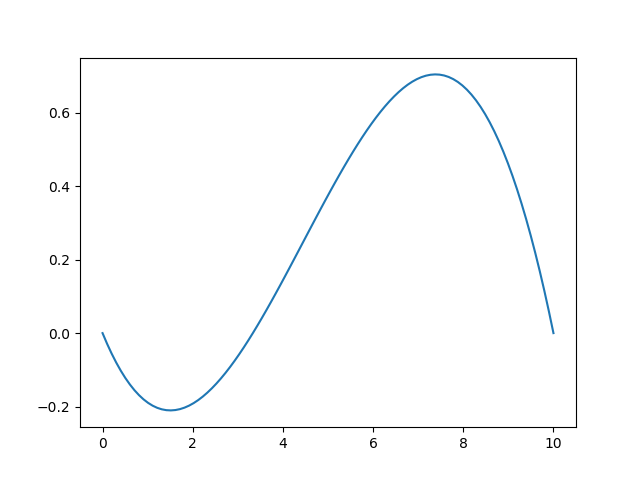
\includegraphics[scale=0.6]{polynominal.pdf}
        \caption[Polynomial of the Replicator Dynamic]{$\varphi(x)$ for the parameter setting $a=5, b=0, c=4, d=3$}
        \label{fig:polynomial}
\end{figure}
A solution through an initial state $x_0$ of the dynamical system is called a 
\textit{trajectory}, whereby it is distinguished between a forward trajectory 
for $t \rightarrow \infty$ and backward trajectory for $t \leftarrow \infty$.
Analytic solutions, i.e.\ solutions one can express with the use of
basic functions, can only be derived for simple cases. 
However, the existence and uniqueness of a solution through
any initial state for the replicator dynamic is guaranteed by the theorem 
of \textit{Picard-Lindel\"of}, theorem 6.1 in 
\textcite[74]{weibull_evolutionary_1997}. 

Once a solution is obtained, the question whether there 
is a connection between the evolutionary dynamic and the equilibria in the 
stage game arises. To see this, consider the concept of a fixed point.
A point $\vec{x}^*=(x^*_1,x^*_2)^T \in \realnumb^2$ of a dynamical system, such as the replicator 
dynamic in equation \eqref{eq:replicator}, is called a fixed point
if $\dot{\vec{x}} = 0$ at $\vec{x}^*$ , i.e.\ it stays in the 
current state for all $t \rightarrow + \infty $. 
Analyzing equation \eqref{eq:replicator}, 
this happens if either a strategy
is not present in the population or the excess payoff of a strategy is zero. 
Consequently, considering equation \eqref{eq:replicatorpara}, in the stag 
hunt game a fixed point can be characterized by an $x^*$ for which
$\varphi(x^*) = 0$.
The fixed points of the dynamic coincide 
with the Nash equilibria of the stage game as 
$\varphi(x^*) = 0$ for $x^* \in \{0,\frac{\alpha_2}{\alpha_1+\alpha_2},1\}$. 
It suffices to calculate the roots of the polynomial $\varphi(x)$, either
numerical or, as the Nash equilibria are usually calculated beforehand,
reducing the degree by polynomial division. 

In general, the replicator 
dynamic lacks the \textit{Nash stationarity} property and thus there are 
games with fixed points which are not a Nash equilibrium
\parencite{sandholm_population_2010}.
For a trivial example, consider the prisoner's dilemma in figure \ref{fig:pd}. 
A population consisting only of cooperating agents stays in that state
which is not a Nash equilibrium forever. However, inserting one single 
defecting agent would lead all other agents to imitate the strategy defect,
as it has a higher payoff, so that in the end the whole population defects.
Therefore, one is usually interested in the fixed points of 
a dynamical system that are stable in terms of some 
disturbance of the system. 

A quite strict and useful concept of stability, often used in evolutionary 
game theory, is \textit{asymptotic stability}. 
It essentially requires that a system in a specific fixed point returns 
to the fixed point after a perturbation.
Hence, the system tends to move back to an asymptotically stable fixed point
once disturbed. Formally, an $\epsilon$-perturbation of 
$\dot{x} = \varphi(x)$ is a trajectory of the system with the initial
condition $x_0$ in some ball $B_\epsilon(x^*)$ of radius $\epsilon >0$ and 
$x_0 \neq x^*$. 
In one dimension a ball $B_{\epsilon}(x)$ is simply an interval 
$[x^*-\epsilon, x^*+\epsilon]$ around the fixed point $x^*$.
The fixed point $x^*$ is then called \textit{asymptotically
stable} if there exists an $\epsilon$-perturbation for which $x(t) \rightarrow
x^*$ as $t \rightarrow \infty$. 
The \textit{basin of attraction} of a fixed point $x^*$ is defined as the set 
of points $x_0 \in \realnumb$ for which a trajectory through $x_0$ approaches 
the fixed point $x^*$. For the one dimensional case, 
this is simply the interval 
of $x$ for which any solution to the differential equation with the initial 
conditions in this interval converges to the fixed point. With the following 
theorem independently contributed by \textcite{hartman_lemma_1960} and 
\textcite{grobman_homeomorphism_1959}, one can easily 
find the asymptotically stable fixed points in the stag hunt game:
\begin{mydef}
        If a one dimensional dynamical system $\dot{x}(t) = \varphi(x)$ 
        has a hyperbolic fixed point $x^*$, $x^*$ is asymptotically stable
        if its linearization 
        $\dot{x} = \varphi'(x^*)x$ at that fixed point 
        is asymptotically stable, with
        $\frac{\partial \varphi(x)}{\partial x}:= \varphi'(x)$.
        A fixed point is called hyperbolic in one dimension if 
        $\varphi'(x^*) \neq 0$. The linearization is stable at that
        point if $\varphi'(x^*) < 0$ and not stable if $\varphi'(x^*) >0$.
\end{mydef}
The solution to the linearization can be analytically derived by 
a standard tool for differential equations - separation of variables and 
integration.
Accordingly, the linearization around the fixed point $x^*$ is 
$x(t)= x_0 e^{\varphi'(x^*)t}$, where $x_0=x(t=0)$ denotes the 
initial condition, i.e.\ the share of agents choosing strategy 1 in the 
beginning.
Applying the theorem to equation \eqref{eq:replicatorpara}, 
one finds that the 
fixed point $x=0$, corresponding to the Nash equilibrium of hunting hare, is 
asymptotically stable, since $\varphi'(0) = - \alpha_2 <0$. 
The linearization around the fixed point is $x(t) = x_0 e^{-\alpha_2 t}$, 
which clearly approaches zero as $t \rightarrow \infty$. 
Similarly, the Nash equilibrium 
of hunting stag at $x=1$ is an asymptotically stable fixed point as
$\varphi'(1) = -\alpha_1 <0$ with linearization $x(t) = x_0 e^{-\alpha_1 t}$.
At the inner fixed point one gets 
$\varphi'(\frac{\alpha_2}{\alpha_1+\alpha_2}) = 
\frac{\alpha_1 \alpha_2}{\alpha_1+\alpha_2} >0$. By the linearization theorem
the inner fixed point is not asymptotically stable.
In general, more sophisticated mathematical tools such as the theorem of 
Lyapunov and entropy functions are needed to prove whether a fixed point
is asymptotically stable \parencite{friedman_economic_1998}.

Another way to look at the asymptotic stability of the inner fixed
point is the following.
Suppose the population is currently at the inner fixed point and now 
some agents come from outside into the population
using strategy 1, represented by the share $\epsilon$,
$\frac{\alpha_1}{\alpha_1+\alpha_2}>\epsilon > 0$.
The new population state is 
$x_{\epsilon}=\left(\frac{\alpha_1}{\alpha_1+\alpha_2} + \epsilon\right)$.
An asymptotically stable fixed point is now expected to withstand the invasion
and make the outsiders imitate the prevailing strategy composition. Hence, 
the change of the population share $\dot{x}$ should be negative.
Plugging $x_{\epsilon}$ into
\eqref{eq:replicatorpara} one finds that $\dot{x} >0$, the population share
choosing strategy 1 grows for every $\epsilon >0$, converging to the 
fixed point $x = 1$. Conversely, for an invasion by a share $\epsilon$ 
of agents
choosing strategy 2, $0 > \epsilon > \frac{\alpha_2}{\alpha_1+\alpha_2}$,
agents start switching away from strategy 1 to strategy 2 $(\dot{x} < 0)$ 
and hence, the population share of agents playing strategy 1 
decreases, until it reaches the 
fixed point $x=0$. 
Hence, only population state which involve the play of an ESS are asymptotically 
stable.

The key things to remember are that, a Nash equilibrium is a rest point of
the replicator dynamic. Furthermore, not all rest points are 
Nash equilibria in general. And finally, strict Nash equilibria 
are asymptotically stable. These results do not just hold for
the evolutionary stag hunt game, but are true for the replicator dynamic
in general. In the literature these connections between the stage game
and the replicator dynamic are summarized in the
\textit{Folk Theorem of Evolutionary Game theory} 
\parencite[25]{szabo_evolutionary_2007}. Interestingly, every payoff
monotone dynamic satisfies this theorem, as shown in 
\textcite{hofbauer_evolutionary_2003}, and hence, many dynamics have the same
dynamic properties for the stag hunt game. 

In figure \ref{fig:basinofattraction} the graph of the replicator dynamic
in the stag hunt game for $\alpha_1=1$ and $\alpha_2=3$ are plotted. The
horizontal axis represents time $t$, while the vertical axis shows
the share of the population choosing strategy 1. The dashed gray horizontal
line represents the inner fixed point of the dynamic at $75\%$.
Red trajectories converge to the population state $x=0$, the hare hunting
equilibrium, whereas blue trajectories converge to the population state in 
which all agents hunt stag.
\begin{figure}
 \centering
        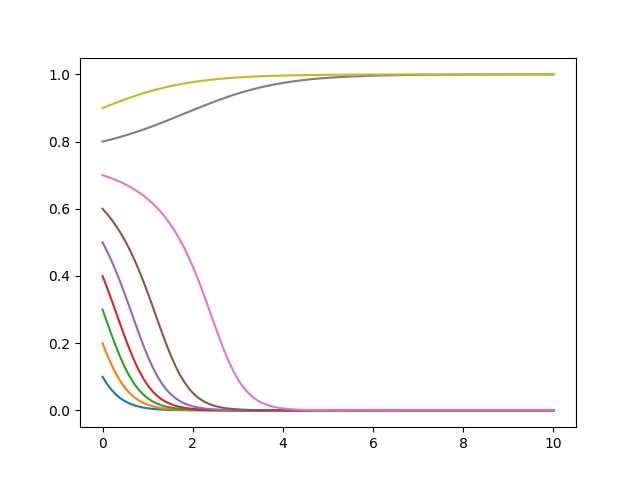
\includegraphics[scale=0.6]{basinofattraction.pdf}
        \caption[Replicator Dynamic of the Stag Hunt Game]{Replicator dynamics in the stag hunt game for 
                $\alpha_1=1,\ \alpha_2=3$ with different initial conditions}
                \label{fig:basinofattraction}
\end{figure}

Concerning the equilibrium selection, the evolutionary approach with replicator
dynamic has a definite answer. The population will be in one of the three
Nash equilibria depending on the initial condition after some time. 
However, an equilibrium that is not asymptotically stable 
is rather implausible,
because it only emerges from one initial condition in which the population
is already exactly in that population state. 
Intuitively, one additional agent playing
a pure strategy suffices to get the population state moving to one of the
pure equilibria. As the model outlined here is only a deterministic
approximation, any stochastic shock would lead to such a disturbance and hence
would start convergence to one of the states with evolutionary stable 
strategies.
The population converges to the stag hunting or the hare
hunting equilibrium if the initial conditions lie in their 
basin of attraction.
As discussed earlier, the population converges to the state $x=1$, 
the stag hunting equilibrium of the stage game, for all initial conditions 
$x_0 \in (\frac{\alpha_2}{\alpha_1+\alpha_2},1]$. Any trajectory of the 
dynamical system with initial conditions 
$x_0 \in [0,\frac{\alpha_2}{\alpha_1+\alpha_2})$ leads to the hare hunting
equilibrium. 

Interestingly, one observes another connection of the 
dynamic with the stage game. 
By definition \eqref{eq:riskdom}, 
the hare hunting equilibrium risk-dominates if $\alpha_2 > \alpha_1$.
Thus, the basin of attraction is larger for an equilibrium that 
risk-dominates the other. With the parameter setting shown
in figure \ref{fig:basinofattraction}, $75\%$ of the possible initial 
conditions lead to the risk-dominant equilibrium, whereas only $25\%$ of 
them lead to the payoff-dominant equilibrium. This 
connection was for example also shown by \textcite{kandori_learning_1993} 
in a stochastical model. The convergence to the risk-dominant equilibrium
in one dimension was independent of the specific adjustment process 
underlying the dynamic, as long it satisfied payoff monotonicity. 
However, it is not clear what specifies the 
initial conditions which ultimately determine the selected equilibrium in 
the deterministic case. 
If it is assumed, for example, that agents choose a random strategy 
in a first round of the game independently from each other, 
one can say that the equilibrium with a 
larger basin of attraction, the risk-dominant equilibrium, is reached more 
likely. Otherwise, a ``slice of history'', knowledge about how the population
has played before, is needed to know in which population
state the dynamic starts \parencite{friedman_economic_1998}. 

%
%
%%%%%%%%%%%%%%%%%%%%%
%
%
% Network externality
%
%
\section{Coordination and Network Externalities}
\label{sec:simplemodel}
This section investigates the effect of a network externality on the
evolutionary stag hunt game. The following situation is inspired by an
example given in \textcite{kandori_learning_1993}. 
Consider students in university being assigned to
projects in their classes with other students at university. 
Nowadays, most of the projects involve some kind of software tool to either 
present the results, analyze the subject or just manage the process of aggretating 
knowledge. Usually the choice of the tools can be simplified to 
the choice of proprietary software or open source software. 
For reasons of simplification, assume that both 
software types are capable of producing
the same quality of ouput for the projects and are similiarly easy to handle.
The only difference is the high license cost for proprietary software.
Common examples of this are Open Office vs.\ Microsoft Word for text editing,
Python vs.\ Matlab for scientific computing and R vs.\ Stata for statistical
analysis. Assigned to a project, students can either choose proprietary
software denoted as strategy 1 or open source software denoted as strategy 2.
If both students choose open source software they receive utility $(a)$.
Coordinating on propierty software leaves both with a utility $(d)$ which is
smaller than $(a)$ as they have to pay for the licenses. In the case 
where students fail to coordinate on a software tool, the student
with proprietary software gets $(c)$. However, the other student
has to transfer his contributions to the standards of the proprietary software
as portability is usually only possible in this direction.
Hence, this stundet only gets $(b)$. The parameters fullfill 
the condition $a > c \geq d >b$.
Evidently, the structure of the game is precisely that of a stag hunt game. 
Coordination on open source software is the payoff-dominant Nash equilibrium,
but it is risk-dominated by the equilibrium in which the students 
coordinate on proprietary software. 

For simplification, assume that during their studies, a large body of 
homogenous students is randomly paired by their professor into groups of two 
for a project, implicitly playing the coordination game outlined. 
Concerning the behavior of an individual student, I assume that they are 
not perfectly rational and do not adjust their software choice 
each time they have to do a project.
For simplicity, students in this model behave according to the 
revision protocol of pairwise proportional imitation discussed in section 
\ref{sec:revisionprotocols}. 
This applies as students tend to use software they always used and 
only change it, if they get to know someone being more successful with
another software choice. Therefore, the dynamic in the model can be 
described by the replicator dynamic derived for the stag hunt game in 
equation \eqref{eq:replicatorpara}.
This model would not differ in terms of convergence and stability of Nash 
equilibria to the evolutionary stag hunt game above.

However, I want to introduce \textit{network externalities} in this model. 
The interest of the economic literature turned to open source software 
development, because it is commonly observed that users contribute to 
programming projects without receiving a monetary compensation for it.
In fact users share their source code publicly to the open source community,
being motivated by peer recognition and the signaling for career concerns
\parencite[21]{lerner_simple_2002}.
The utility for a student increases with the size of the community as 
more students contributing code enhance the variety and usefulness of the 
software. 
To incorporate this in the model, let the utility for a student 
in the case of coordination on open source software be a function of 
population size using that strategy $f(x)$. 
Preserving the general structure of the
game, it is useful to focus on the functional specification 
$f(x) = a + e(x)$, where $(a)$ is the payoff parameter used 
previously and $e(x)$ denotes the network externality. 
A positive network externality satisfies $e(x)\geq 0$ and 
$\frac{de(x)}{dx}>0$, 
as an increase of the population share choosing the strategy
also increases the utility due to the network. 
Including the parameter $(a)$ ensures that the utility of this 
strategy combination is never below the utility of coordination on 
proprietary software. Otherwise, the structure of the stage game would 
differ fundamentally with respect to the population share choosing strategy 1. 

The payoff matrix, using local shifts, is 
$A=\begin{psmallmatrix}\alpha_1+u(x) && 0 \\ 0&& \alpha_2\end{psmallmatrix}$. 
Substituting into the replicator dynamic  \eqref{eq:replicatorpara} yields:
\begin{alignat}{2}
        \dot{x} = \varphi(x) = x^2(\alpha_1+e(x) +2\alpha_2 ) 
        - x^3(\alpha_1+e(x)+\alpha_2) - x(\alpha_2)
        \label{eq:externalitymodel}
\end{alignat}
By plugging $x=0$ and $x=1$ into equation \eqref{eq:externalitymodel} and 
by applying the linearization theorem, one can ensure 
that the fixed point with pure strategies and their
property of asymptotical stability did not change
($\varphi'(1) = -\alpha_1 -e(1),\ \varphi'(0) = -\alpha_2 -e(0)$).
The literature on network externalities usually assumes a diminishing
marginal effect of the network externality $\frac{d^2e(x)}{dx^2} <0$ 
\parencite[73]{lin_impact_2008}. However, the analysis presented in this text
will focus on the linear form $e(x) = \beta x$ with the externality parameter
$\beta \in \realnumb_+$. This restriction does not change the main implication
of the model. 
Despite not changing the stability of the pure states, 
the externality affected the inner fixed point of the dynamic.
The polynominal $\varphi(x)$ is now of degree $4$:
\begin{align}
        \dot{x} = \varphi(x) = -\beta x^4 -x^3(\alpha_1 + \alpha_2 
        - \beta ) + x^2 (\alpha_1 + 2 \alpha_2) - x(\alpha_2)
\end{align}
Using the knowledge from the general case, we can find the roots, i.e. fixed
points of the dynamic, by reducing the degree with the two roots known. The
polynominal of degree $2$ can then be solved applying a quadratic formula\footnote{
The solution with negative sign was omitted, since it has no economic 
interpretation.}, so that the fixed point with a mixed population state is
$x_3 = -\frac{\alpha_1+\alpha_2}{2 \beta} + 
\sqrt{\frac{(\alpha_1+\alpha_2)^2}{4\beta^2} +\frac{\alpha_2}{\beta}}$. 
The new inner fixed point is always lower than the inner fixed point without 
externality. It cannot coincide with the stag hunt equilibrium, as it 
satisfies $0<x_3<\frac{\alpha_2}{\alpha_1+\alpha_2}$. 
Taking the limit $\lim_{\beta \rightarrow 0} x_3 = 
\frac{\alpha_2}{\alpha_2+\alpha_1}$ verifies the intuition that for a 
diminishing network externality parameter $\beta$ the model without 
externality is obtained.
The plot of the dynamic and the polynominal is 
shown in figure \ref{fig:plotmodellinear}.
Note that the share of students choosing strategy 1 is now lower at the 
inner fixed point, displayed by the gray dashed lines in subfigure 
\ref{fig:externalitypolynominal}, showing that the externality has a positive 
effect on the attractiveness of choosing open source software. 
Using the argument developed above, the inner fixed point is still not
asymptotically stable. Any feasible share of outsider $\epsilon$ 
with a pure strategy would lead to convergence to one of the 
pure population states as $|\varphi(x_3+\epsilon)|>0$.
Indeed, the basin of attraction of the equilibrium in which all 
students are using open source software became larger, 
depicted by the distance to the inner fixed point.
This is illustated by the dashed, red horizontal line, 
the inner fixed point without externality, and the dashed, green horizontal 
line, the inner fixed point with externality, 
in figure \ref{fig:dynamiclinear}.
\begin{figure}[h]
        \centering
        \begin{subfigure}{.5\textwidth}
        \centering
        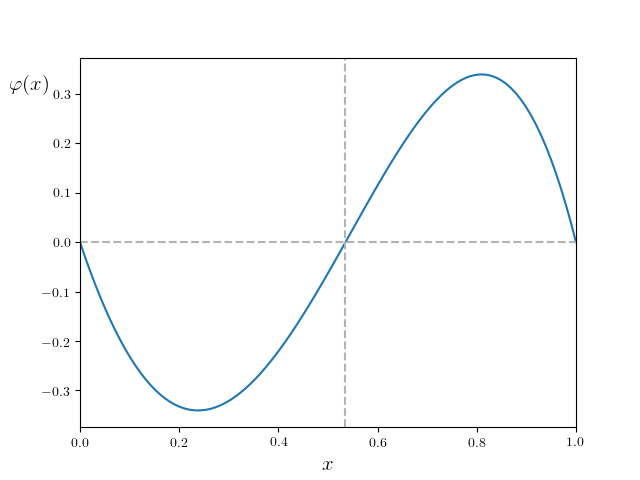
\includegraphics[scale=0.5]{polynominallinearmodel.pdf}
        \caption[Polynominal of the externality model]{The polynominal $\varphi(x)$} 
        \label{fig:externalitypolynominal}
        \end{subfigure}%    
        \begin{subfigure}{.5\textwidth}
        \centering
        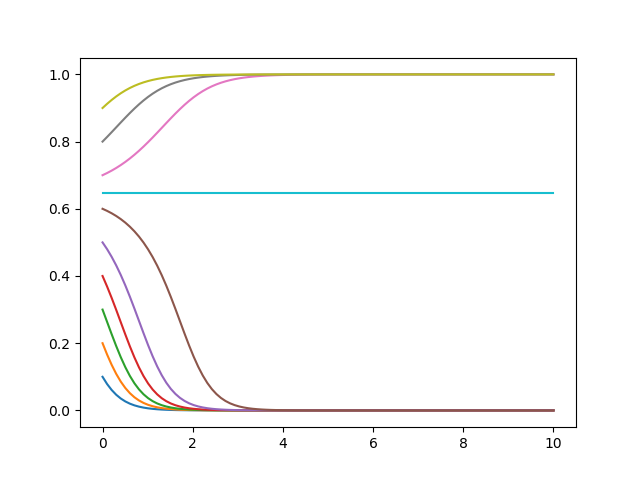
\includegraphics[scale=0.5]{dynamiclinearmodel.pdf}
        \caption[Replicator dynamic of the model with externality]{The dynamic $x(t)$ for different $x_0$} 
        \label{fig:dynamiclinear}
        \end{subfigure}%        
        \caption[Polynominal and Dynamic of the model with externality]
        {The linear externality 
                model for parameters $\alpha_1=1,\alpha_2=3,\beta=3$}
        \label{fig:plotmodellinear}
\end{figure}
The basins of attraction have equal size for $\beta^* = 2 (\alpha_2 -\alpha_1)$,
attracting an equal amount of initial conditions. However,
the proprietary equilibrium looses its risk-dominance property 
only for $1 > x > \frac{\alpha_2-\alpha_1}{\beta}  $, using definition 
\ref{eq:riskdom}. The right hand side of the equation must be lower than one 
to make a change of the risk-dominance property feasible. In this model,
the size of the basins of attraction and the risk-dominance
property do not coincide in general, since the externality affects the Nash 
product associated with the pure strategy 1 equilibrium. Consider for example 
the parameter setting $\alpha_1 =1, \alpha_2=3$, and $\beta=3$ in figure 
\ref{fig:plotmodellinear}. 
The basins of attraction are not equal, since $3<\beta^*= 4$. 
All trajectories starting with 
$x_0 \in (\frac{-2+\sqrt{13}}{3},1]$ converge to the open source equilibrium
and hence the proprietary equilibrium attracts
all trajectories with $x_0 \in [0,\frac{-2+\sqrt{13}}{3})$. 
Clearly, the latter basin of 
attraction is larger ($\frac{-2+\sqrt{13}}{3}>0.5)$, 
but the open source equilibrium gets risk-dominant for
$x>\frac 23$. This implies that the network externality not only increases the
utility obtained from the choice of open source software, but also,
combined with a high enough user base, makes this choice risk-dominant. 

The model presented here is a simplification of the real world. 
First, the students are expected to be able to review which software is 
appropriate for their projects, hence have more information available than 
assumed in the model. Secondly, talking to their fellow student seems
possible before deciding which software to use for the project. 
However, as the experimental literature that will be discussed in section 
\ref{sec:experimentalevidence}, and \textcite{aumann_nash_1990} suggest, 
cheap talk does not generally solve the coordination problem. 
Additionally, the way the payoff of a strategy increases with
the population size using it, the network externality, 
is modeled quite naively.
Students at university and social networks in general are not fully
connected as students, for example, only do projects with fellow students
in the same classes. Furthermore, students usually try to do projects
with people they are socially connected with. In fact, the assumption about
a fully connected network is ``one of the main criticisms of evolutionary game
theory'' \parencite[246]{hanauske_evolutionare_2011}. 
As a consequence, many researchers recently gave attention to the 
structure of the network underlying the interaction of agents and 
evolving of network structure \parencite[46]{szabo_evolutionary_2007}.
For example, \textcite{ohtsuki_simple_2006} found 
that fewer connectivity 
leads to more cooperation for a range of network topologies,
agreeing with the intuition
``The fewer friends I have the more strongly my fate is bound to theirs'' 
\parencite[1]{ohtsuki_simple_2006}.
Additionally, \textcite{santos_evolutionary_2006} found in a model with
a heterogenous population with respect to the links of each agent that 
cooperation on the payoff-dominant outcome is easier to achieve than
in a fully connected population.
Although the model with a positive linear network externality is far too 
simple to capture the effect of complex, adapting networks, it gives an 
intuition of how coordination of a small group, in this case two players, 
can be affected by the choice of the whole population, as it changes
the structure of the coordination game they play.

%
%%%%%%%%%%%%%%%%%%%%%
%
%
% Experimental section
%
\section{Experimental Evidence}
\section{Experimental Evidence}
\label{sec:experimentalevidence}
A third approach beside the traditional and the evolutionary treatment of 
coordination problems is what \textcite{camerer_behavioral_2003} calls the 
'fundamental empirical' approach.
Hence, this section consults the experimental economic literature regarding 
laboratory coordination games to provide evidence how actual people choose
their strategies in such situations and which factors might influence them. 
Precisely, do people, if they are able to coordinate on an equilibrium at all,
play the risk-dominant or the payoff-dominant equilibrium? And how does their
choice change playing the game repeatedly?
Due to the rich experimental literature on coordination in social 
dilemmas, the focus will be on studies with framework close to  
evolutionary SH game. A comparison will show the shortcomings and what
is described well by the evolutionary framework.
 
Due to the different notations authors use, a translation into the present
notation was performed.
On these grounds, the 
strategy used in the payoff-dominant equilibrium of the SH game will be 
either called  \textit{strategy 1} or in analogy to the stag hunt story 
\textit{hunting stag}.
Consistently, the strategy used in the risk-dominant equilibrium is called
\textit{strategy 2} or \textit{hunting hare}. 

The papers of \textcite{van_huyck_tacit_1990} and 
\textcite{cooper_communication_1992} are seen as the first experiments 
investigating coordination games \parencite{devetag_when_2007}.
In \textcite{van_huyck_tacit_1990}, subjects do not play a stag
hunt, but an order-statistics game. These games differ in that subjects can
choose from a broader set of strategies and hence there are more than two 
equilibria in the game. The games are played in a group and the payoff to 
all players depend on the lowest strategy one of them chose, thus the name 
'weak-link' order statistics game. Nevertheless, the structure is similiar to
the stag hunt in the way that the equilibria are Pareto-ranked, with one 
'safe' strategy \parencite{devetag_when_2007}.
So evidence from this games is 
likely to be transferable to the coordination problem in the stag hunt game. 
In \textcite{van_huyck_tacit_1990} subjects played the order-statistics 
game in 
groups of 14-16 for 10 periods. They only received information about their 
payoff, but that was sufficient for the players to find out what the 
lowest choice of one subject in 
their group was. Astonishingly, in every experiment the groups converged
to the equilibrium with the lowest payoff. 
This result were preserved in another 
five periods of this game although the subjects played an alternative payoff
matrix embracing the payoff-efficient equilibrium across all groups 
inbetween. 
Replications of this results have been performed numerously, with 
varying group sizes and slightly changed payoff matrices 
\parencite[6]{devetag_when_2007} 
\textcite{cooper_communication_1992} used a
two-player stag hunt game\footnote{They call 
it simple coordination game (SCG).}  
and one augmented by a dominated strategy. They found that 
subjects in randomly matched one-shot games, knowing only about their own
received payoffs, also fail to coordinate without any preplay communication. 
However, they find that two-way communication, in which both players were
able to send a message to their matched partner containing which strategy
they intend to choose, solves the coordination problem in the SCG. 
Against the hypothesis of \textcite{aumann_nash_1990}, the messages
apparently contained useful information for the players, but only if both
were able to communicate.
However, the 
early approaches suggest that without cheap talk 
coordination failure\footnote{Here in the meaning of not being 
able to coordinate on the payoff-dominant equilibrium} 
is common in the laboratory \parencite[2]{devetag_when_2007}. 
It is noteworthy that the studies 
discussed use different matching protocols, fixed matching in groups and 
random matching against one other player, and yet found the same results. 
As a consequence, experimentalists focused mainly on the characteristics 
of the payoff matrix instead of implementational details in laboratory SH 
games \parencite[8]{devetag_when_2007}.

\subsection{Variation of the payoff matrix}
The implementation of random matching in a group closely resembles the 
evolutionary setting discussed in section \ref{sec:evolutionarystaghunt}, 
because a group of players, repeatedly matched in pairs, play the stag hunt 
game, having only information about their own payoff and the payoff their
opponents used. Certainly, it is to suspect that real players, opposed
to the programmed agents in the evolutionary setting, are able to remember
what the other players chose in the rounds before. \todo{historyofplay}

Random matching was conducted by \textcite{battalio_optimization_2001}. 
Subjects played three stag hunt games with the typical symmetric pure strategy
equilbrium and the symmetric mixed strategy equilibrium at $(0.8,0.2) \in
\Delta$. Figure \ref{fig:payoffbattalio} shows the payoff matrices of the
games $2R, R$ and $0.6R$ used. The names become clear when observing the 
\textit{optimization premium} of the games. While controlling for the basin of 
attraction of the equilibria - the mixed equilibrium is equal in all games -
they want to explore the effect of an increase in the ``premium for playing
a best-response'' \parencite[751]{battalio_optimization_2001}. 
In order to investigate this, they define the optimization premium $r_j(y)$ of 
a game $j$ as the difference in payoffs choosing the pure strategies 
$e_1$ and $e_2$ while expecting the opponent to play a strategy 
$y=(q,1-q)^T \in \Delta$:
\begin{align}
        r_j(y)= \hat{F_j}(e_1,y) - \hat{F_j}(e_2,y) = \delta_j(q-q^*),
\end{align}
with the \textit{optimization premium parameter} $\delta_j$. In the notation
 of the parametrized SH game, $\delta_j = a - c + d - b$.
The parameters for the payoff matrices are reported in figure 
\ref{fig:payoffbattalio}. 
First of all, they find support for their hyptohesis that in games with a 
larger optimization premium subjects coordinate less frequently on the 
payoff-dominant equilibrium. 
Contrary to game $0.6R$, where only one cohort coordinated according 
to risk-dominance, in $2R$ no cohort and in $R$ only one cohort 
converged to the payoff-dominant equilibrium. The replicator dynamic does 
not offer a description of this behavior, since convergence to an 
equilibrium only depends on its basin of attraction once the dynamic 
started, which do not differ for the three games. 
Whereas ``all 24 cohorts start in the basin of attraction
of the risk-dominant equilibrium'' 
\parencite[755]{battalio_optimization_2001}, all should converge to the 
risk-dominant equilibrium according to the dynamic.
In most cases this is true, with only two exceptions in game $0.6R$ 
and one $R$.
But, for the sake of completness, a crossing of the  
``best-response separatrix'' \parencite{battalio_optimization_2001} i.e. 
mixed-strategy equilibrium, can not happen in the deterministic replicator 
dynamic. Furthermore, as they conjectured, a larger optimization premium 
increases the speed of convergence. Hence, a coordination on a equilibrium 
was achieved fastest in the $2R$ game. This is consistend with a 
postulated replicator dynamic for this games. Starting from 
\eqref{eq:replicator}, one can derive that the dynamics of this 
games are the same up to a change in speed, proportional to the ratio of 
optimization premia of the games. In game $R$ the change in the population share
playing strategy one is, thus, half the speed of $2R$ and four thirds of $0.6R$,
$\dot{x}_{R} = \frac 12 \dot{x}_{2R} = \frac{4}{3}\dot{x}_R$.

\textcite{schmidt_playing_2003} designed their experiment such that the effect
of differing risk levels could be observed. It is convenient to relabel 
the strategies in the game, because in their treatment the payoff-dominant 
equilibria is in the right corner of the normal form game representation,
contrary to the notation used throuhout this text. Comparing risk levels between
games, they used a measure due to \textcite{selten_axiomatic_1995}, defined
as:
\begin{align}
        \label{riskmeasureschmidt}
        R = ln\left(\frac{\hat{F}(e_2,e_2) -\hat{F}(e_2,e_1)}{\hat{F}(e_1,e_1) 
        -\hat{F}(e_2,e_1)}\right) = ln \left(\frac{d-b}{a-c}\right).
\end{align}
The risk measure $R$ is positive, if the Nash equilibrium $(e_2,e_2)$ is
risk-dominant, and negative if the payoff-dominant equilibrium inhibits both
properties.
None of the four games in \textcite{schmidt_playing_2003} handles
the case of $R=0$, where the mixed-strategy equilibrium is risk-dominant.
In difference to \textcite{battalio_optimization_2001}, they do not
use the proposed optimization premium, but rather measure the risk-dominance 
level in relative terms as $P=\frac{a-d}{a}$.\footnote{As they mention, the 
games in \textcite{battalio_optimization_2001} vary in their level of 
P accordingly.}
The payoff matrices of the games are shown in \ref{fig:payoffschmidt}.
Comparing game 2 with game 3, and game 1 with game 4, the 
only difference is the degree of risk-dominance and hence one can 
investigate if subjects react to the change in risk-dominance. 
For game 1 and game 3 the basin of attraction of both equilibria is equal 
(Mixed-NE at $(\frac 12, \frac 12)$) and  for
game 2 and 3 the Mixed-NE is at $(\frac 34,\frac 14)$ resulting in the 
typical  larger basin of attraction of the strategy $(e_2,e_2)$. 
Therefore, it is expected from the replicator dynamic, of course 
depending on the inital condition 
of the game, that subjetcs are more likely attracted to the 'hare-hunting' 
equilibrium in game 2 and 3.
\textcite{schmidt_playing_2003} implemented three different types of matching
protocol. First of all, a random matching protocol where each subject is not
matched twice with another person and only has information 
about his payoff and the action of the person he was matched against. 
Secondly, a fixed protocol, matching two persons for several rounds against 
each other, followed by a series of one-shot games. 
In the random matching protcol, they find evidence that an increase in 
risk-dominance, i.e. an increase in $R$, leads to a higher choice of the
strategy in the risk-dominant NE.\todo{Schmidt et al paper.} 

\textcite{dubois_optimization_2012} conducted a similiar experiment as 
\textcite{schmidt_playing_2003} and \textcite{battalio_optimization_2001},
but introduced a different measure for the risk subjects are confronted with in
the games. They defined the \textit{relative riskiness} of a games 
``safe strategy relative to the risky strategy'' as $RR = \frac{|c-d|}{a-b}$. 
\todo{Hier Zitation?}
Intuitively, a player commited to strategy one and calculating the 
difference a deviation of the other player from strategy one to two, gets
$(a-b)$. Similiary for strategy two, he receives $(c-d)$. The relative riskiness
measure is, hence, the ratio of the effect a deviation of the other play has 
on the payoff. Alternatively, it can be interpreted as the ratio of the 
standard deviations of the payoffs 
\parencite[372]{dubois_optimization_2012}. 
They speak of ``comparable riskiness'', if the $RR$ measure is close to one 
\parencite[372]{dubois_optimization_2012}. 
According to $RR$, the risk-dominant 
strategy 2 is said to be less risky, relative to the 
payoff-dominant strategy in a game, if the $RR$ is smaller.
Observing the values of the relative riskiness by 
\textcite{dubois_optimization_2012} and the risk-dominance measure of 
\textcite{schmidt_playing_2003} for the games used in the papers, it is clear
that both measures are in a conflict. As by \textcite{schmidt_playing_2003}
\todo{possessivcite}
measure, risk-dominance is kept constant in the games of 
\textcite{battalio_optimization_2001}, whereas relative riskiness indicates a
variation. On the other hand, relative riskiness cannot distinguish between
the games 1,2 and 3 of \textcite{schmidt_playing_2003}, since $RR=0$. In an
early working version of their paper they explicitly excluded the case 
$c \neq d$ and statet that ``a more general measure of relative riskiness 
should allow for the case where c=d as compared to $(a-b)$'' 
\parencite{dubois_optimization_2008}. 
\todo{Maybe both measures capture different things: Intuition}
Game 1 replicated \textcite{battalio_optimization_2001}'s 
game\footnote{The payoff matrices are identical} $0.6R$ (Compare \ref{fig:payoffdubois} and \ref{fig:payoffbattalio}). 
As per their conjecture, they found that a lower relative riskiness 
in a game decreases the rate players choose strategy one, 
keeping the optimization premium constant. This is congruent with 
the intuition that the severity of the impact related with the 
strategic uncertainty subjects face in a game, expressed in
the difference in payoff a deviation of the other player would cause,
effects the choice of the strategy. 
On the other hand, keeping the relative riskiness constant and varying the
optimization premium, they cannot find an effect on the frequency of 
strategy 1. 
In measuring the ``coordination sucess'', they deploy the concept of ``strong
coordination''. 
In other words, counting the occurence of periods in which a group
uniformly adopts a strategy such that every pair of subjects lands in one
of the Nash equilibria. \textcite{dubois_optimization_2012} intend to sort 
out ``furtuitous coordination'', coordination as consequence of subjects being
randomly matched with each other \parencite[373]{dubois_optimization_2012}.
Comparing strong coordinations between the games they find a non-significant 
difference between game 1 and game 2 in which only the relative riskiness 
ceteris paribus was changed. Contrary to that, there is a significant 
difference in the commonness in game 3 to game 2.
Since game 3 and 2 only differ in their optimization premium, 
\textcite{dubois_optimization_2012} conclude that a higher optimization
premium leads to more frequent (strong) coordination. 
As they mention, this agrees with the observation of 
\textcite{battalio_optimization_2001} that coordination success depends 
positively on the optimization premium. 

As seen from the evidence \textcite{battalio_optimization_2001},
\textcite{schmidt_playing_2003} and \textcite{dubois_optimization_2012} 
found, the structure of the payoff matrix has a strong impact on the way 
people play the stag hunt game.   
The story this evidence tells is quite frightening. Failure to coordinate 
on the payoff-dominant equilibrium seems to be common. 
Following an argument of \textcite{kreps_game_1990} that identical strategic 
interactions, such as the play of completely indentical stag hunt games 
in the laboratory, ``take us very little distance outside the laboratory'' 
\parencite[212]{kreps_game_1990}, 
\textcite{rankin_strategic_2000} design an experiment with a randomly 
pertubated stag hunt game. Essentially, the payoff to strategy 1 is fixed 
whereas the payoff to strategy 2 varies randomly between the games. This is
depicted in the payoff matrix \eqref{eq:payoffrankin}.
\begin{align}
        \label{eq:payoffrankin}
        A = \mqty(1 & 0 \\ x & x)
\end{align}        
The parameter $x$ is equally distributed between $(0,1)$ and, once a sequence
was calculated, used for all cohorts participating in the experiment. This
variation justifies to describe the games as ``similiar'' but not
``identical'', hence the structure stays the same, but the risk-dominance 
property varies. Indeed, if $x$ is greater than $0.5$ risk-dominance and
payoff-dominance select different equilibria, $(e_2,e_2)$ and $(e_1,e_1)$,
respectively. For a value of $x$ smaller than $0.5$ both select 
the equilibrium in strategy 1. One finds that the optimization premium for 
this randomly perturbed games does not change, since $\delta=1-x+x+0=1$. 
The relative riskiness measure $RR$ cannot discriminate between this games,
since $|d-c|=0\ \forall x$. \textcite{schmidt_playing_2003} measure of risk of 
course is positive for $x > 0.5$ and negative for $x <0.5$. 
\todo{how to cite?}
The question \textcite{rankin_strategic_2000}
want to investigate is, if this framework of sligthly varied situations may
lead the groups to form a ``convention'' which deductive principle to choose. 
In contrast to the studies performed with identical stag hunt games, they 
observe coordination to the payoff dominant equilibrium across
all cohorts. Whereas in the first ten periods of play risk dominance seems
to have some explanatory power for the choice of strategy, in the last ten
rounds 91\% choose the payoff dominant action. 
In the cases of coinciding equilibrium selection of risk-dominance and 
payoff-dominance ($x < 0.5$) all subjects coordinated on that equilibrium in 
group 1-5 and 95\% of the subjects in group 6. But also for the other case a 
high coordination on the payoff-dominant strategy was observed, ranging from 
80\% to 95\% of the strategies played, suggesting that there is clear evidence
for the hypothesis of an emerging convention based on the deductive principle
payoff-dominance. This sends a quite positive image about coordination, because 
this is ``dramatically at odds with claims that coordination failure is common''
\parencite[9]{devetag_when_2007}. 
As outlined, most studies concerned with the stag hunt game in the 
laboratory focused on the characteristics of the payoff matrix. 
However, implementational details 
such as the matching protocol influence behaviour sharply. Not only 
\textcite{van_huyck_tacit_1990} found in their two-player fixed matching
convergence to the payoff-dominant equilibrium, 
\textcite{clark_repetition_2001} also found different strategy 
choices between randomly matched one-shot games and fixed matching protocol 
games. The latter lead to significantly higher choices of the strategy 
in the efficient equilibrium and less ``disequilibrium play'' in general
\parencite[]{clark_repetition_2001}. 
\textcite{devetag_when_2007} mention that one-shot games imply a 
random matching protocol. But it is different to random matching on group
basis, where subjects can play against the same opponent again 
and hence there is the possibility that a ``convention'' emerges like in 
\textcite{rankin_strategic_2000}.

Even more subtle experiment design differences are conjectured to have an
effect. For example \textcite{devetag_when_2007} suggest that the formulation
``you will remain grouped with the same seven other participants for the next
75 rounds'' in the instruction of the \textcite{rankin_strategic_2000}  
experiment may increased trust within the group and hence was a 
cause for the exceptional coordination success. Comparatively, the 
instructions in \textcite{dubois_optimization_2012} read ``At the beginning
of each period, in each group (composed of 8 participants), the computer
system will form 4 pairs of subjects. [...] The experiment 
involves 75 rounds''\parencite[378]{dubois_optimization_2012}. 
While essentially containing the same information,
it does not emphasize the fact that subjects can reencounter the same 
players again and consequently might have influenced the subjects to play
the strategy associated with less risk.

An interesting experimental approach is executed by 
\textcite{dufwenberg_gender_2005}. They tried to evaluate whether 
there is a difference in coordination behavior accross genders, motivated by 
the different treatment of males and females in the work place. Playing the 
weak-link order statistics game in \cite{van_huyck_tacit_1990}, groups of 
only females or only males face the coordination problem with Pareto-ranked 
equilibria. The motivation of observing gender differences was 
``never explicitly pointed  out to the subjects'' 
\parencite{dufwenberg_gender_2005}\footnote{
Even though it might be interesting to see if there is an effect like 
the discussed ``crab basket'' effect which leads woman to mistrust each other 
more than in a mixed group.}. However, they did not find that the groups play
different. Differences in the beginning ``disappeared fast and no difference
is found in later stages'' \parencite[235]{dufwenberg_gender_2005}. 
All groups converged to the choice of the minimum
contribution. As they mention, it might be useful to investigate differences
with groups that also have some other characteristica in common. They refer
to the differences group identity has for females and males playing a 
public goods game. Namely, \textcite{croson_groups_2008} found that when
females in a sorrority play the public goods games they perform better than 
females with no specific belongingness. Contrarly, males in a fraternity 
performed worse than males without a group identity. 
Interestingly, this and other factors concerning the group of subjects 
playing the coordination game might be a rationale for the initial conditions
in the evolutionary dynamic. The intitial conditions might be used to 
capture the composition of the subjects interacting, reflecting how well
trust or cultural conventions are embedded in the population. 
Nevertheless, it seems difficult, atleast for the author, to justify
the reduction of the inheritance of cultural values to one\footnote{Of course, 
in games with more than two strategies the initial conditions are represented 
by a vector} dimension such as the initial conditions $x_0$.

The discussion of the laboratory research makes on clear: There is more
to the coordination problem than individuals programmed like a robot 
to a strategy, while being attracted and moved to an equilibrium by a dynamic
in a fully deterministic fashion. But, as a model should, the analysis offers 
a simplification that helps to understand some of the patterns observeable 
when real people interact. 

%
%
%
%%%%%%%%%%%%%%%%%%%%%
%
%
% Summary and Outlook
%
\section{Conclusion}
%%%%%%% 
%%
%% Summary and Outlook
%%
%%%%%%%

Answering the question which factors affect social cooperation, one might
only be able to give a partial answer. 
This is because the problem of cooperation can occur due to different
reasons.
The origin of the dilemma described in this thesis is the uncertainty 
of individuals about their counterparts choice. 
While one outcome guarantees everyone a higher 
payoff, they may fear that the other player deviates and hence, also choose 
the safer option. 
In the social sciences, the most frequently used framework for social dilemmas
involves a conflict between the individual interest and the interest of 
the group.
However, Camerer, for instance, argues that various situations that 
``are thought to be a prisoner's 
dilemma are actually a stag hunt game'' 
if the described situation ``is likely enough to be repeated, evokes emotion, 
has enough synergy or excludability'' 
\parencite[376-377]{camerer_behavioral_2003}. Hence, the 
stag hunt game finds a wide range of different applications,
for example the coordination in the macroeconomy \parencite{bryant_coordination_1994}, 
publishing decisions in academia \parencite{hanauske_evolutionare_2011} and
in the discussion of the social contract \parencite{skyrms_stag_2004}.

The empirical evidence considered in section \ref{sec:experimentalevidence}
suggests that failure to coordinate on the payoff-dominant 
outcome for the group in pure stag hunt games is common. 
In general, even preplay communication does not solve this.
However, situations in the real world that can be treated as a coordination
game may not involve the identical structure all the time. The
results of \textcite{rankin_strategic_2000} suggest that people can learn 
to coordinate when confronted with variation and hence, we might not
have to be that pessimistic about coordination.
Evolutionary game theory does not describe all varieties of the 
behavior in the laboratory. As a model should, it offers a simplification
that helps to understand some of the patterns observable when real people
interact. Additionally, it emphasizes that for a wide range
of behavioral rules coordination on the risk-dominant equilibrium
is more likely. While applied in various disciplines such as biology, 
psychology and political science, for example 
\textcite{friedman_economic_1998} argues that the full potential
of evolutionary game theory for economic applications 
has not yet been unlocked. He suggests that "economists must re-adapt
evolutionary theory to economics" before it will be widely accepted 
\parencite[18]{friedman_economic_1998}. The underlying concept of behavior and
the simplification of an infinite population have to be carefully reflected
when applying the framework to economic problems. Furthermore, questioning
the structure of the population is important, as the underlying social
network may be pivotal for coordination success.

%
%
%%%%%%%%%%%%%%%%%%%%

\newpage
\printbibliography
\newpage
\begin{appendices}
\setcounter{figure}{0}
\renewcommand\thefigure{\thesection.\arabic{figure}}    
\section{Games of the Experimental Literature}
\begin{figure}[H] \hspace*{\fill}
        \begin{subfigure}{0.3\textwidth}
                \begin{game}{2}{2}[$\delta_{2R}=50$]
                & $S$ & $H$ \\
            $S$ & $45,45$ & $0,35$ \\
            $H$ & $35,0$  & $40,40$ 
    \end{game} \hspace*{\fill}%
    \caption{Game $2R$}
    \end{subfigure}
    \begin{subfigure}{0.3\textwidth}
            \begin{game}{2}{2}[$\delta_{R} = 25$]
            & $S$ & $H$ \\
       $S$  & $45,45$ & $0,40$ \\
       $H$  & $40,0$ & $20,20$ \\
       \end{game} 
       \caption{Game $R$}
       \end{subfigure}
       \begin{subfigure}{0.3\textwidth}
               \begin{game}{2}{2}[$\delta_{0.6R}=15$]
            & $S$ & $H$ \\
       $S$  & $45,45$ & $0,42$ \\
       $H$  & $42,0$ & $12,12$ \\
       \end{game}
       \caption{Game $0.6R$} 
       \end{subfigure}
\caption{Games used in \textcite{battalio_optimization_2001}}
\label{fig:payoffbattalio}
       \end{figure}
       \baselineskip
       \vspace{20mm}
\begin{figure}[H] 
        \begin{subfigure}[b]{0.5\textwidth}
                \centering
                \begin{game}{2}{2}[$P=\frac 25$, $R=0$]
                & $S$ & $H$ \\
            $S$ & $100,100$ & $20,60$ \\
            $H$ & $60,20$  & $60,60$ 
    \end{game} 
    \caption{Game 1}
    \end{subfigure}
    \begin{subfigure}[b]{0.5\textwidth}
            \centering
            \begin{game}{2}{2}[$P=\frac 15$, $R=ln(3)$]
            & $S$ & $H$ \\
       $S$  & $100,100$ & $20,80$ \\
       $H$  & $80,20$ & $80,80$ 
       \end{game} 
       \caption{Game 2}
       \end{subfigure}
       \vskip\baselineskip
       \begin{subfigure}[b]{0.5\textwidth}
               \centering
               \begin{game}{2}{2}[$P=\frac 15$, $R=0$]
            & $S$ & $H$ \\
       $S$  & $100,100$ & $60,80$ \\
       $H$  & $80,60$ & $80,80$ 
       \end{game}
       \caption{Game 3} 
       \end{subfigure}
       \begin{subfigure}[b]{0.5\textwidth}
               \centering
            \begin{game}{2}{2}[$P=\frac 25$, $R=ln(3)$]
            & $S$ & $H$ \\
       $S$  & $100,100$ & $0,80$ \\
       $H$  & $80,0$ & $60,60$ 
       \end{game} 
       \caption{Game 4}
       \end{subfigure}
\caption{Games used in \textcite{schmidt_playing_2003}}
\label{fig:payoffschmidt}
       \end{figure}
       \vspace{2cm}

\begin{figure}[H] \hspace*{\fill}
        \begin{subfigure}{0.3\textwidth}
        \begin{game}{2}{2}[$RR_{Game 1}=\frac 23$]
                & $S$ & $H$ \\
            $S$ & $45,45$ & $0,42$ \\
            $H$ & $42,0$  & $12,12$ 
    \end{game} \hspace*{\fill}%
    \caption{Game 1}
    \end{subfigure}
    \begin{subfigure}{0.3\textwidth}
            \begin{game}{2}{2}[$RR_{Game 2}=\frac 14$]
            & $S$ & $H$ \\
       $S$  & $40,40$ & $20,37$ \\
       $H$  & $37,20$ & $32,32$ \\
       \end{game} 
       \caption{Game 2}
       \end{subfigure}
       \begin{subfigure}{0.3\textwidth}
               \begin{game}{2}{2}[$RR_{Game 3}=\frac 14$]
            & $S$ & $H$ \\
       $S$  & $44,44$ & $4,38$ \\
       $H$  & $38,4$ & $28,28$ \\
       \end{game}
       \caption{Game 3} 
       \end{subfigure}
       \caption{Games used in \textcite{dubois_optimization_2012}}
\label{fig:payoffdubois}
       \end{figure}
       \end{appendices}


\newpage
\thispagestyle{empty}
\section*{Ehrenw\"ortliche Erkl\"arung}
\noindent
Ich versichere hiermit, dass ich die vorliegende Arbeit selbst\"andig und
ohne Benutzung anderer als der angegebenen Quellen und Hilfsmittel verfasst
habe. W\"ortlich \"ubernommene S\"atze oder Satzteile sind als Zitat belegt,
andere Anlehnungen, hinsichtlich Aussage und Umfang, unter Quellenangabe 
kenntlich gemacht. Die Arbeit hat in gleicher oder \"ahnlicher Form noch 
keiner Pr\"ufungsbeh\"orde vorgelegen und ist nicht ver\"offentlicht. Sie
wurde nicht, auch nicht auszugsweise, f\"ur eine andere Pr\"ufungs - oder 
Studienleistung verwendet. Zudem versichere ich, dass die von mir 
abgegebenen schriftlichen (gebundenen)Versionen der vorliegenden Arbeit mit 
der abgegebenen elektronischen Version auf einem Datentr\"ager
inhaltlich \"ubereinstimmen.
\vspace{1cm}

\noindent
Frankfurt am Main, den  \hspace{3cm} Unterschrift:
\end{document}







